\chapter{Configuring your MEGA65}
\label{cha:configuring}

\section{Important Note}

For your convenience, your MEGA65 comes with an SD card with all of the essential
files already on it, so you may prefer to skip this section and jump straight to
the on-boarding section on page \pageref{onboarding}.

Alternatively, you're welcome to read this section and familiarise
yourself on how your SD card was prepared.

{\bf Do not format the SD card that came with your MEGA65}.
If you want to create a new bootable SD card, please use another one,
and keep the SD card that came with your MEGA65 as a safety backup.

\section{Formatting SD cards}
\index{SD Cards!Formatting}
The MEGA65 has two SD card slots: A full-size SD card slot inside, under
the trap-door, and a microSD size slot on the rear.  The current version
of the MEGA65 firmware only supports the use of one SD card at a time.
If you have cards in both slots, the MEGA65 will default to the external slot. The exception to this is that the MEGA65's FDISK/FORMAT
utility can access both, allowing you to select which SD card to format or
repair.

If you wish to use a different SD card to the pre-configured one supplied with your MEGA65, the new SD card must be formatted first.

{\bf This must be done on the MEGA65, not on a PC or other computer.}

{\em Only use SDHC cards. Older SD cards (typically with
  a capacity of <4GB) will not work. Newer SDXC cards with
  capacities greater than 32GB may or may not work. We would
  appreciate hearing your experience with such cards. It is unimportant
  as to which file-system is currently on the card, as the MEGA65
  FDISK/FORMAT utility will completely reformat the card.}

{\bf Why must I format the SD card via the MEGA65 (and not on a PC/computer)?}

There are several reasons for this: First, to fit the most
features into the MEGA65's small operating system, it is
particular about the FAT32 file system it uses. Second, only the
MEGA65 FDISK/FORMAT utility can create a MEGA65 System Partition. The
MEGA65 System Partition holds non-volatile configuration settings for
your MEGA65, and also contains the freeze slots that make it easy to
switch between MEGA65 programs and games.

Formatting an SD card on the MEGA65 is easy. Switch the MEGA65 on while holding \specialkey{ALT} down.

This will present the MEGA65 Utility Menu, which contains a
selection of built-in utilities, similar to the following:

%\begin{wrapfigure}{l}{0.7\textwidth}
\begin{center}
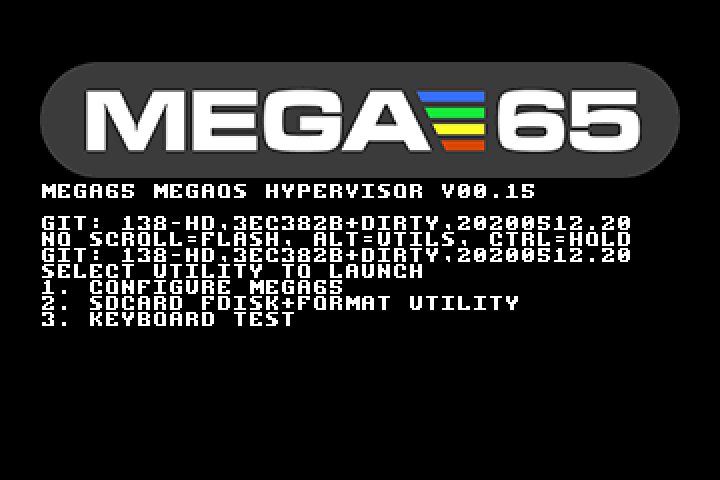
\includegraphics[width=0.7\textwidth]{images/ss-utilmenu.png}
\end{center}
%\end{wrapfigure}

Note that the Utility Menu is always accessible, even if no SD card is present in both the internal and external slots.

The exact set of utilities
depends on the model of your MEGA65 and the version of the MEGA65
factory core which it is running. However, all versions include both
the MEGA65 FDISK/FORMAT utility (which is called \screentext{SDCARD FDISK+FORMAT UTILITY} in the screenshot above),
and the MEGA65 Configure utility.
Most models also include a keyboard test utility, that you can use
to test that your keyboard is functioning correctly.  This is
the same utility used in the factory when testing brand
new keyboards.

Select the number that corresponds to the FDISK/FORMAT utility.  This
will typically be 2.  The FDISK utility will start, and attempt to
detect the size of all SD cards you have installed.  If you have both
an internal and external SD card installed, it will allow you to
choose which one you wish to format. The internal SD card is bus 0,
and the external microSD card is bus 1. Note that the MEGA65 will
always attempt to boot from the external microSD card if one is
present.

For safety, when formatting we {\em strongly} recommend
that you remove any SD card or microSD card that you do not intend to
format, so that you do not accidentally destroy any data.  This is
because formatting an SD card on the MEGA65 cannot be undone, and
all data currently on the SD card {\em will be lost}.  If you
have files or data on the SD card that you wish to retain, you
should first back them up.  The contents of the FAT32
partition can be easily backed up by inserting the SD card into
another computer.  The contents of the MEGA65 System Partition,
including the contents of freeze slots requires the use of specialised
software.

You should aim to back up valuable data from your
MEGA65 on a regular basis, especially while the computer remains under
development.  While we take every care to avoid data corruption or
other mishaps, we cannot guarantee that the MEGA65 is free of bugs in
this regard.

If you have only an internal SD card, you might see a
display similar to the following:

\begin{center}
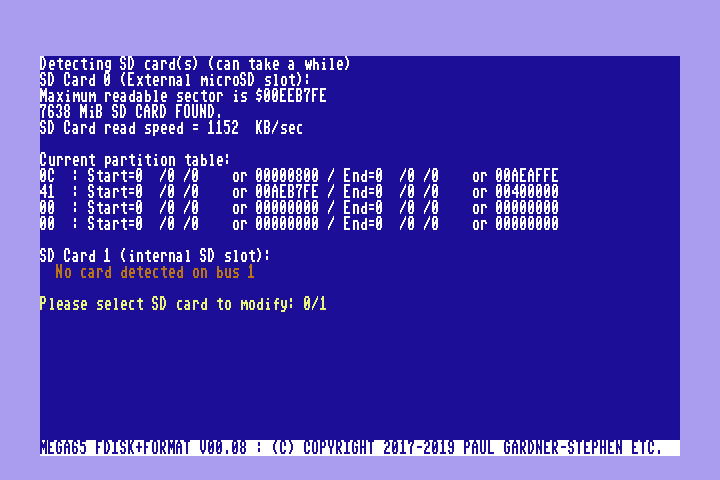
\includegraphics[trim= 10mm  7mm 10mm 10mm,clip,width=0.7\linewidth]{images/ss-m65fdisk-busselect.png}
\end{center}

Once you have selected the bus, the FDISK/FORMAT utility will ask you to confirm that you wish to delete everything:

\begin{center}
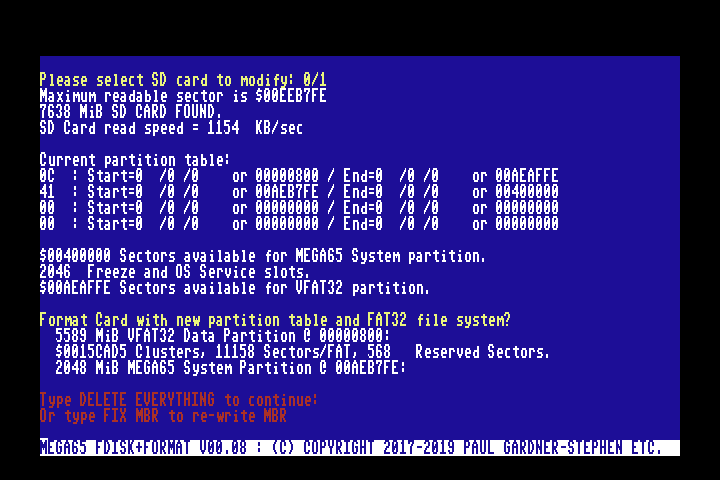
\includegraphics[trim= 10mm  7mm 10mm 15mm,clip,width=0.7\linewidth]{images/ss-m65fdisk-typesomething.png}
\end{center}

To avoid accidental loss of data, you must type \screentext{DELETE EVERYTHING} in capitals and press \specialkey{RETURN}. Alternatively, switch the MEGA65 off and on to abort this process without causing damage to your data.

It is also possible to attempt a recovery from a lost Master Boot Record error (also known as the Boot Sector), by typing \screentext{FIX MBR} instead.

The aim here is to have a correctly formatted SD card with all of the essential files stored on it so the MEGA65 can properly boot.
When switching on, the MEGA65 will search for, and boot using these files:
\begin{itemize}
\item {\tt FREEZER.M65} (Freeze Menu program)
\item {\tt AUDIOMIX.M65} (Freeze Menu audio mixer utility)
\item {\tt C64THUMB.M65} (C64 thumbnail image used in freezer)
\item {\tt C65THUMB.M65} (C65 thumbnail image used in freezer)
\item {\tt MEGA65.ROM}   (128KB ROM file)
\item {\tt MEGA65.D81} (Disk image)
\end{itemize}

Straight out of the box, the MEGA65 will only have one SD card installed, accessible via the trap-door under the case. This SD card contains all of the essential files needed to properly boot up.
If an external microSD card is also detected during boot up, the MEGA65 will give it higher priority, and will try to boot from it instead.
This means that the external microSD card needs to have the essential files on it, otherwise the MEGA65 will not boot up properly and will fall back to loading the OpenROM, which does not support all MEGA65 features.
In general, if your MEGA65 cannot boot properly and falls back to OpenROM, your boot-up screen will look similar to this:

\begin{center}
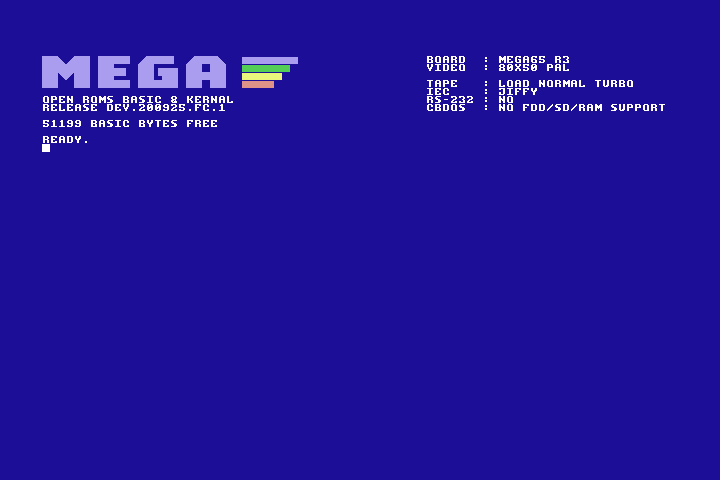
\includegraphics[trim=0 8cm 0 0,clip,width=0.7\linewidth]{images/mega65_OpenROM_boot_noSD.png}
\end{center}


\section{Installing ROM and Other Support Files}
\label{sec:installingrometc}

The MEGA65 FDISK/FORMAT utility will add a copy of the Open ROMs project's C64-compatible ROM
to your SD card, and will name it {\tt MEGA65.ROM}.

For MEGA65 owners, we have replaced this file with the latest ROM from the 'Closed ROMs'
project. It provides many improvements over the original/incomplete C65 ROMs. It contains
the operating system, BASIC 65, CBDOS and the machine language monitor BSMON.
This ROM is developed especially for the MEGA65 and can be
identified by the version number \screentext{92XXXX}.

However, you may have other ROMs that you wish to
use on your MEGA65.
You can copy as many of these as you wish onto the
SD card, just make sure that they have the {\tt .ROM} file extension.  The default ROM
should be called "{\tt MEGA65.ROM}". These files
must be 128KB in size, and use the same internal format as the ROMs
intended for the C65.  This means that the C64-mode KERNAL must be
placed at offset \$E000, a C65-mode BASIC at \$A000, and a suitable
character set at \$D000.

You can optionally name your alternate ROMs as {\tt MEGA65x.ROM}, replacing {\tt x} with a number from 0 to 9.
This allows you to quickly boot-up to your alternate ROMs by holding down a number from \megakey{0} to \megakey{9} prior
to switching on your MEGA65.

Other important support files include {\tt FREEZER.M65} and {\tt AUDIOMIX.M65}, which
allow you to use the MEGA65's integrated Freezer. More details are provided in the
'Floppy Disks, D81 Images, and the Freezer' chapter on page \pageref{cha:freezer}.

\subsection{ROM File}

\textbf{Original C65 ROMs}

You may want to source your own C65 ROM via other means.
There were many different versions created during the development of the Commodore 65,
and the MEGA65 can use any of them.  However, they will not support the advanced
features of the MEGA65, and are incomplete and buggy, as development on them ceased
due to Commodore abandoning the C65 project.

\textbf{MEGA65 Closed ROMs}

There are newer versions of the MEGA65 Closed ROM under development. These ROMs improve upon the original C65 ROMs and make better use of the extra hardware capabilities that the MEGA65 has over the original C65 hardware. These ROMs are available via the filehost (\url{https://files.mega65.org}), but only to owners of the MEGA65, who will need to login to the filehost with their credentials in order to download it. It can be located by visiting the \textbf{Files} tab and searching for "\textbf{kernal rom}":

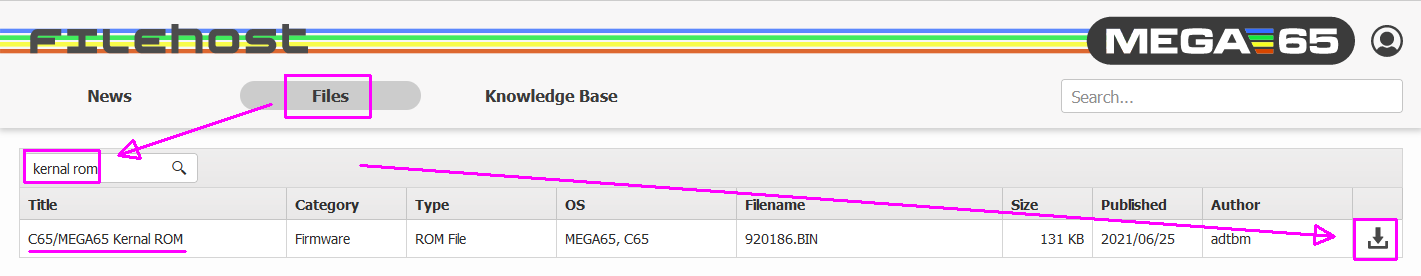
\includegraphics[width=\linewidth]{images/latest_closed_rom.png}

\textbf{MEGA65 ROM diff files}

If you have sourced your own {\tt 911001.bin} C65 ROM and would like to patch it to the latest MEGA65 closed ROM,
we do provide patches, as the additional improvements we have made to the closed rom are open source.
These diff files are available at \url{http://mega65.org/rom-diffs}

\textbf{MEGA65 Open ROMs}

Another available option is to make use of \textbf{MEGA65 Open ROMs}. The latest version of this is always downloadable from either of the following urls:

\begin{itemize}
  \item \url{http://mega65.org/open-roms}
  \item \url{https://github.com/MEGA65/open-roms/raw/master/bin/mega65.rom}
\end{itemize}


\subsection{Support Files}

For official owners of the MEGA65 (both the devkit and the final product), visit the following url and log in with
the user credentials you have been provided. This will take you to the MEGA65 filehost location where the \textbf{MEGA65 SD card essentials} download page is located. Click the \textbf{Download} link to retrieve the latest \textbf{SD essentials.rar} file.

\url{http://mega65.org/sdcard-files}

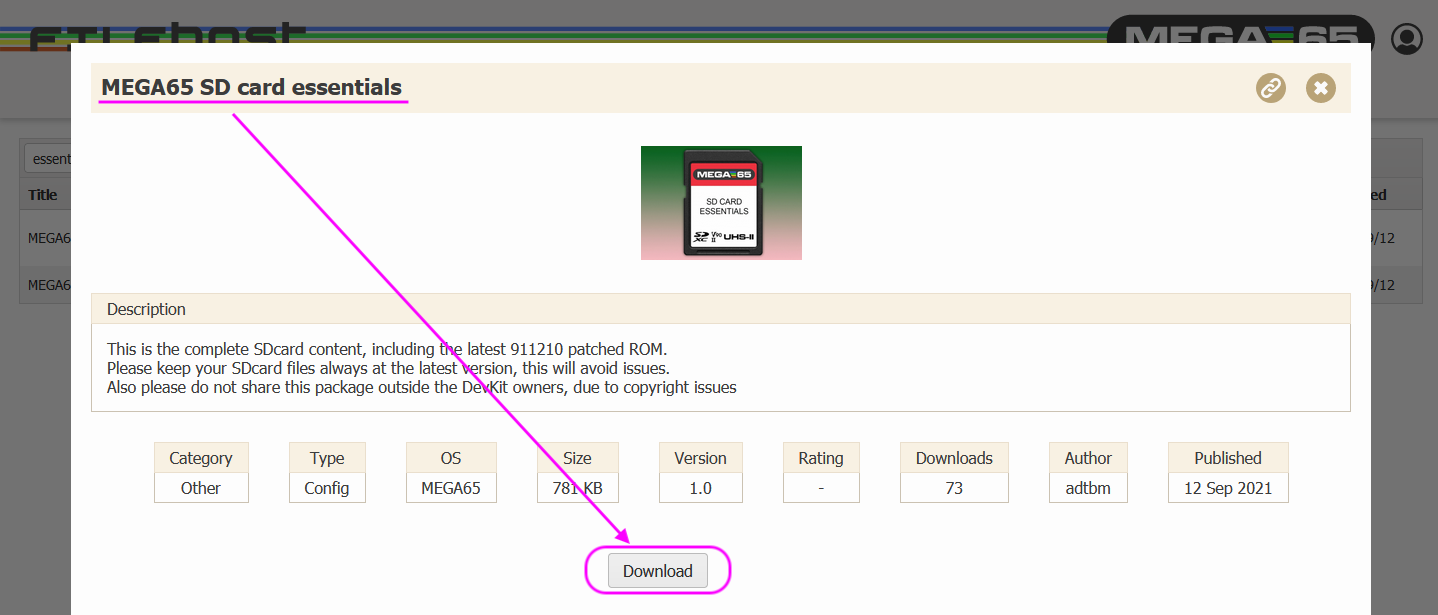
\includegraphics[width=\linewidth]{images/latest_support_files_with_closedrom.png}

Note that this link is only available to official owners of the MEGA65 product, as the fileset also contains the licensed closed-source {\tt MEGA65.ROM} file.
\ifdefined\printmanual
\else
For Nexys board owners in search of a similar fileset (without the ROM), visit the following url instead: \url{http://mega65.org/sdcard-norom}

This will take you to the MEGA65 filehost location where the \textbf{MEGA65 SD card essentials - No ROM} download
page is located. Click the \textbf{Download} link to retrieve the latest \textbf{SD essentialsNoROM.rar} file.

Note that while this fileset does not contain a ROM, there are future plans for it to include the freely available ROM from the Open ROMs project.

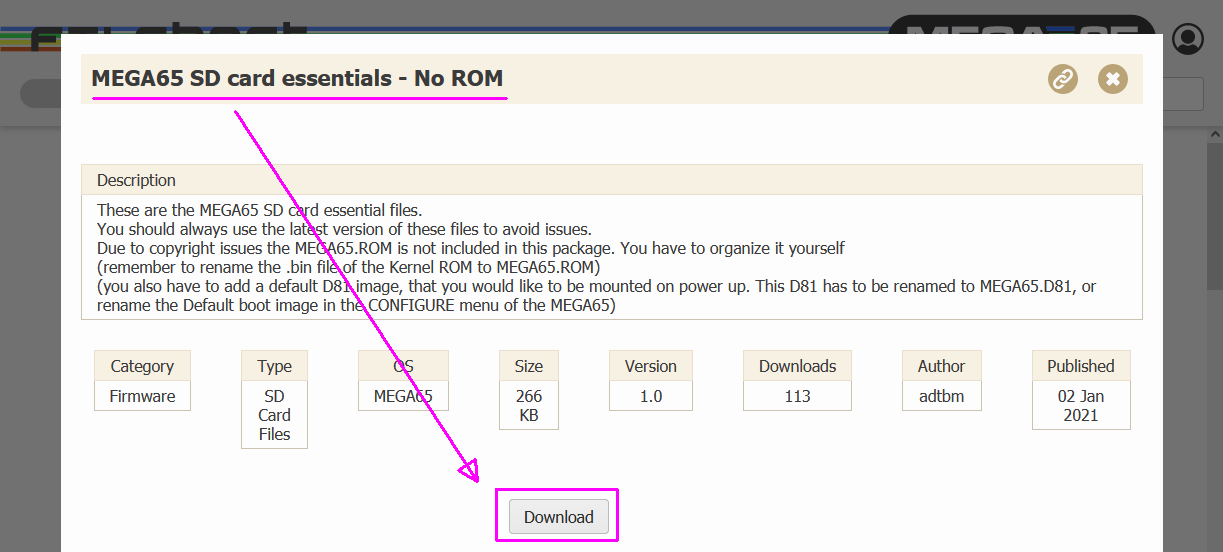
\includegraphics[width=\linewidth]{images/latest_support_files.png}
\fi

\section{On-boarding}
\label{onboarding}

On first launch of your MEGA65, you will see the on-boarding screen:

\begin{center}
  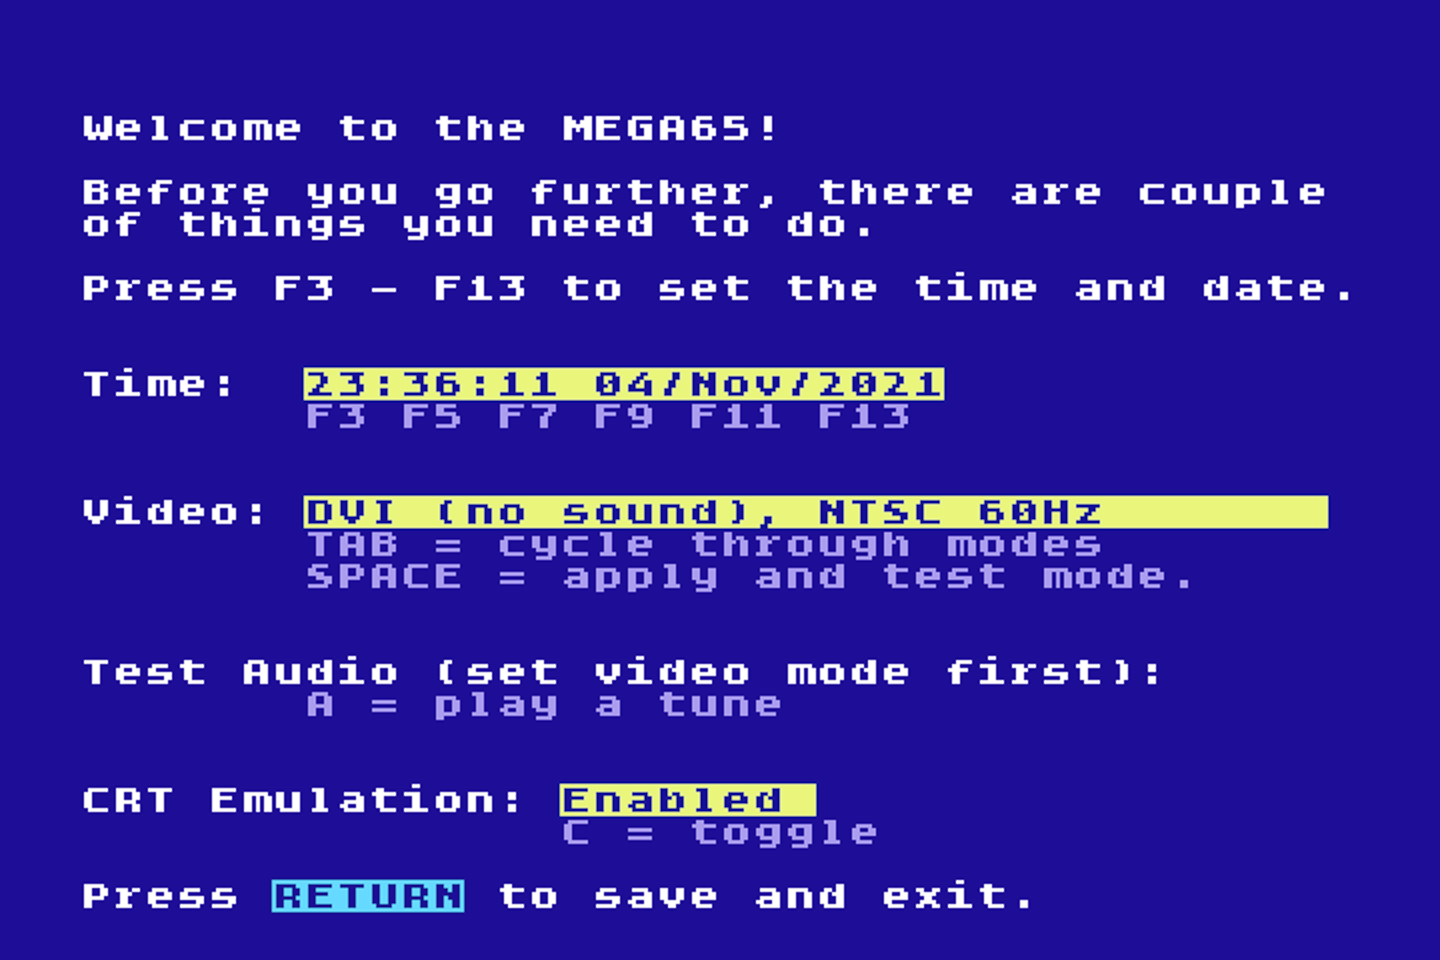
\includegraphics[trim= 10mm 15mm 10mm 10mm,clip,width=0.7\linewidth]{images/img011_final_boot_01.png}
\end{center}

Here you can select and test you screen configuration.

For example, press \specialkey{TAB} to switch to PAL 50HZ:
\index{Display!Setting PAL/NTSC}
\begin{center}
  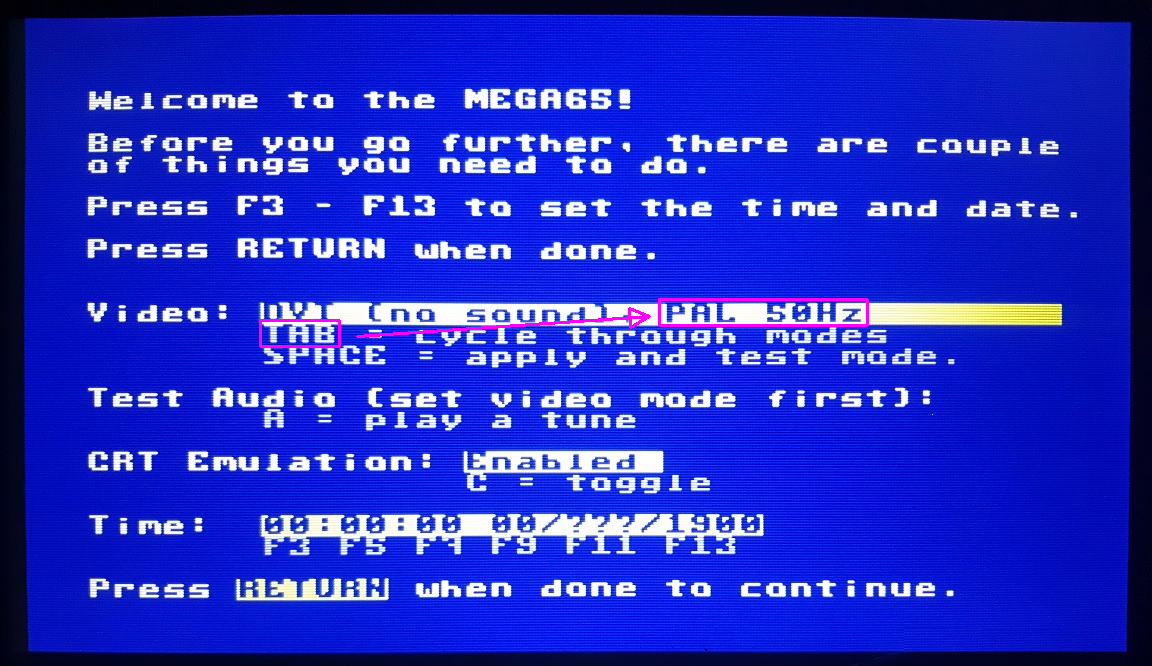
\includegraphics[width=0.7\linewidth]{images/img011_final_boot_02.png}
\end{center}

Then press \megakey{SPACE}, followed by \megakey{Y} to test the new video mode:

\begin{center}
  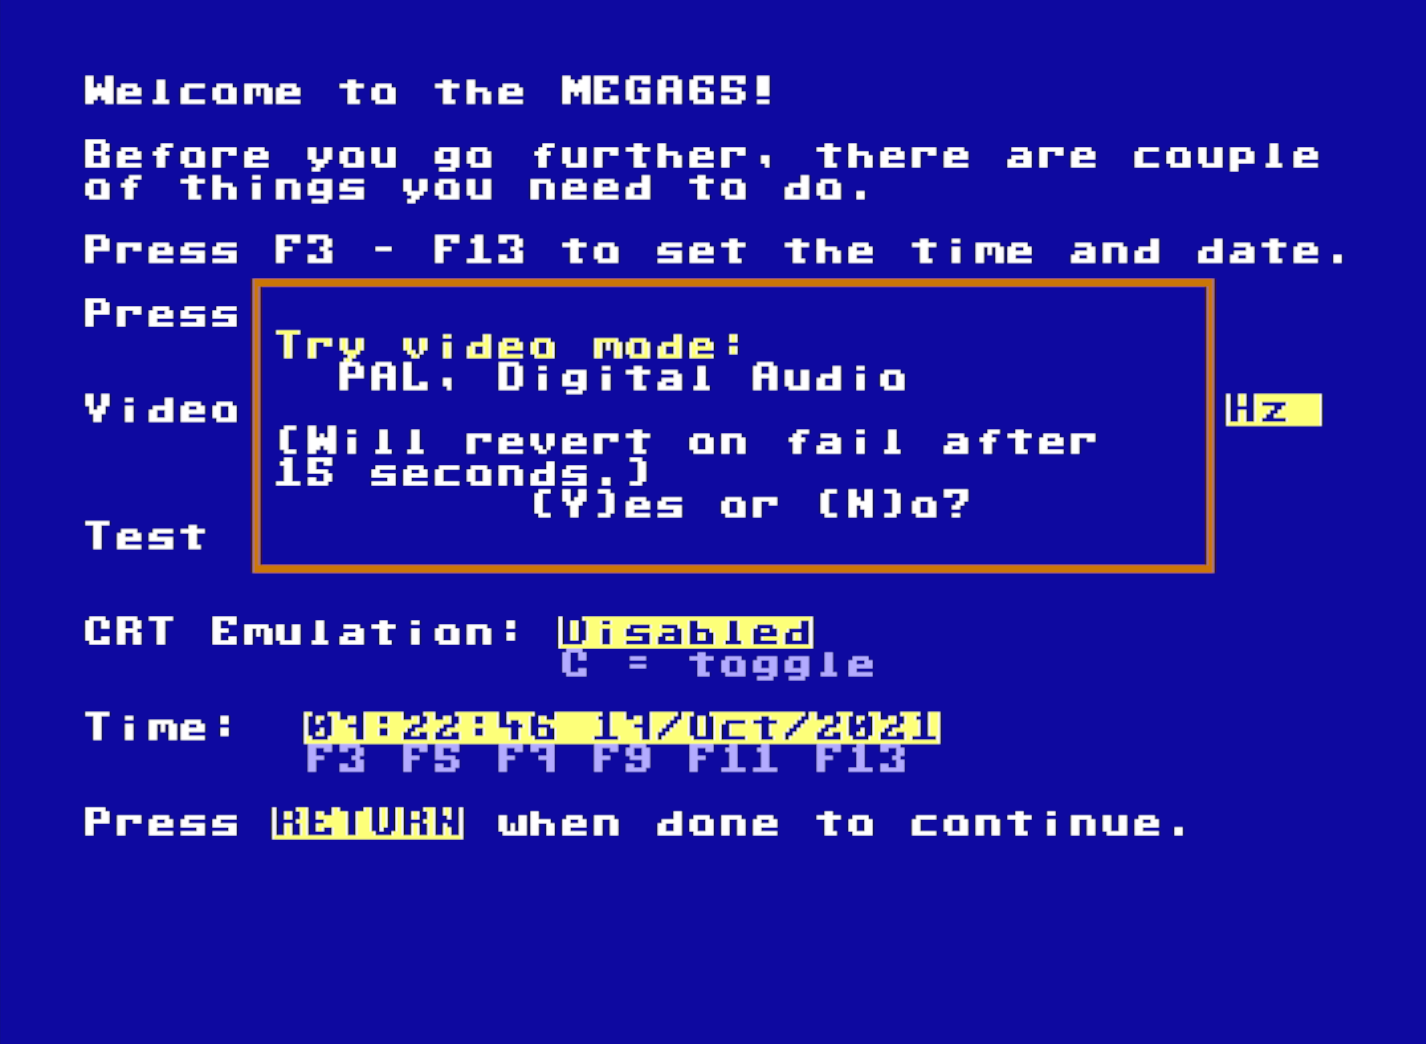
\includegraphics[trim= 15mm 10mm 10mm 15mm,clip,width=0.7\linewidth]{images/img011_final_boot_03.png}
\end{center}

Press \megakey{K} to keep the new video mode:

\begin{center}
  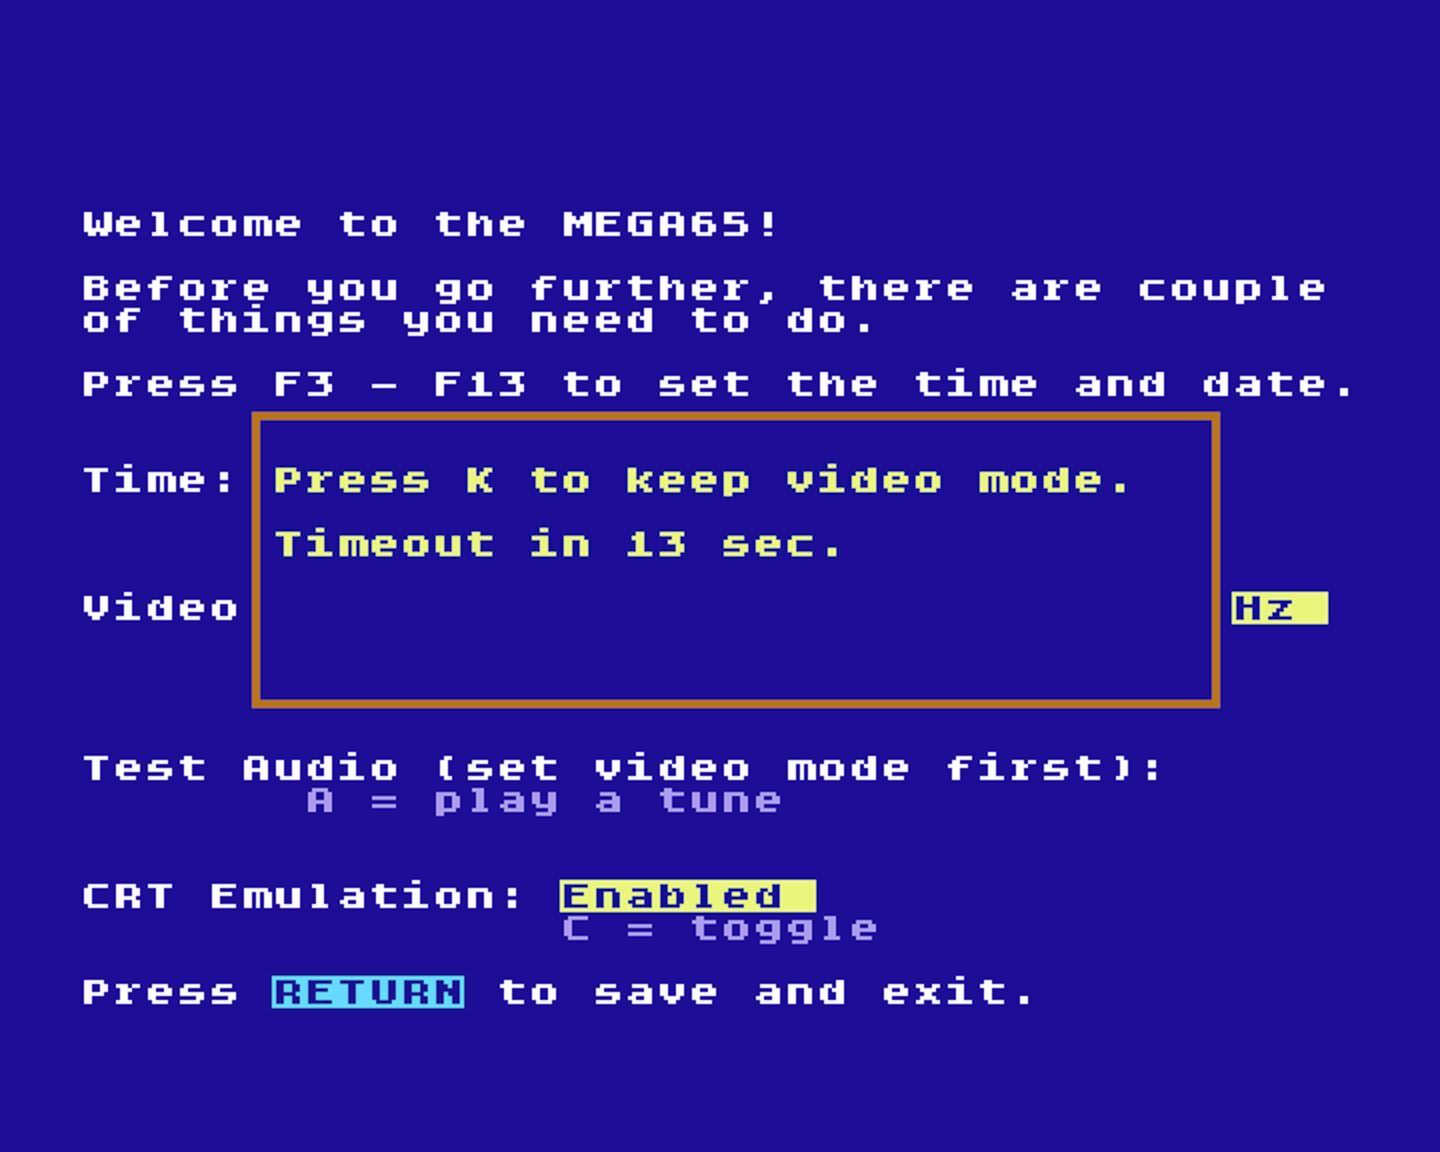
\includegraphics[trim= 20mm 20mm 10mm 25mm,clip,width=0.7\linewidth]{images/img011_final_boot_04.png}
\end{center}

Press \specialkey{RETURN} to complete the configuration:

\begin{center}
  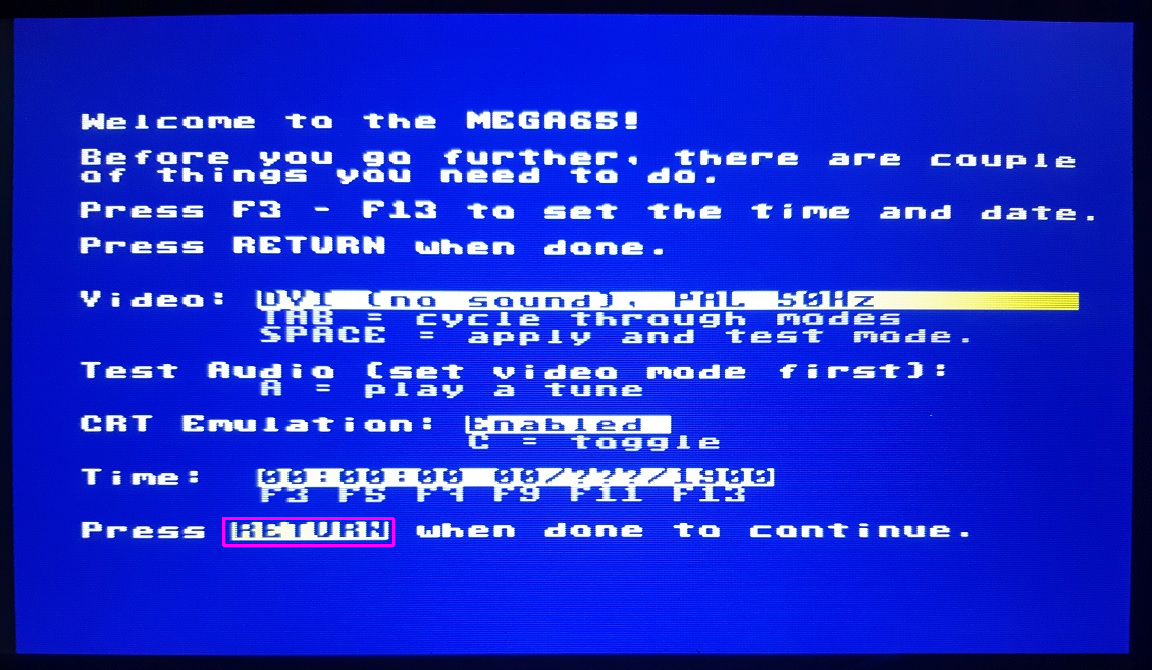
\includegraphics[trim= 6mm 6mm 6mm 6mm,clip,width=0.7\linewidth]{images/img011_final_boot_05.png}
\end{center}

\ifdefined\printmanual
\else
\textcolor{red}{\underline{Note for Nexys4 board users}: \\
\\
  At this very specific step, the board is supposed to reboot and display the main MEGA65 screen. If the board does not reboot and the screen remains black, then switch power to the board off then on again.}
\fi

After the MEGA65 reboots you will be greeted with the main MEGA65 screen:

\begin{center}
  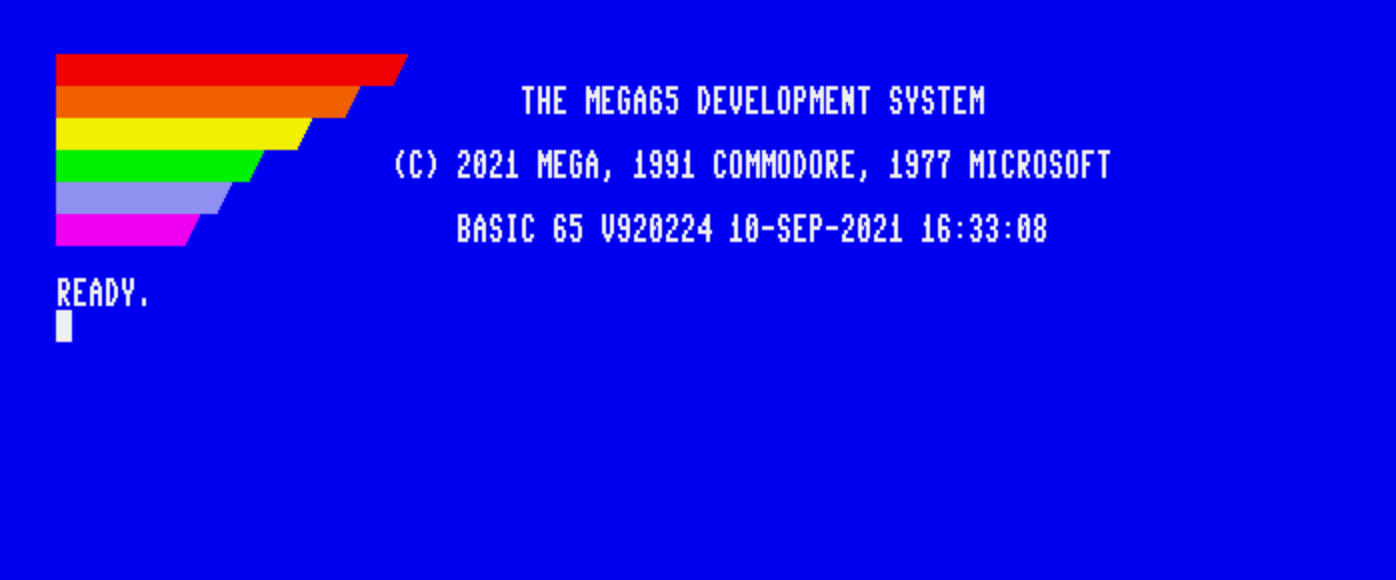
\includegraphics[trim=0 2cm 0 0,clip,width=0.7\linewidth]{images/img011_final_boot_06.png}
\end{center}

\section{Configuration Utility}
\label{sec:configuration-utility}

The configuration utility for the MEGA65 has a similar purpose to the BIOS on a PC, which is to allow you to control certain default behaviours of your MEGA65. However, rather than storing the configuration data in
battery-backed RAM, the MEGA65 stores this data on sector 1 of the SD card. If you switch SD cards, you will change the configuration data.

  To enter the configuration utility, switch the MEGA65 on while
  holding \specialkey{ALT} down.  This will show the utility menu,
  similar to the following:

\begin{center}
  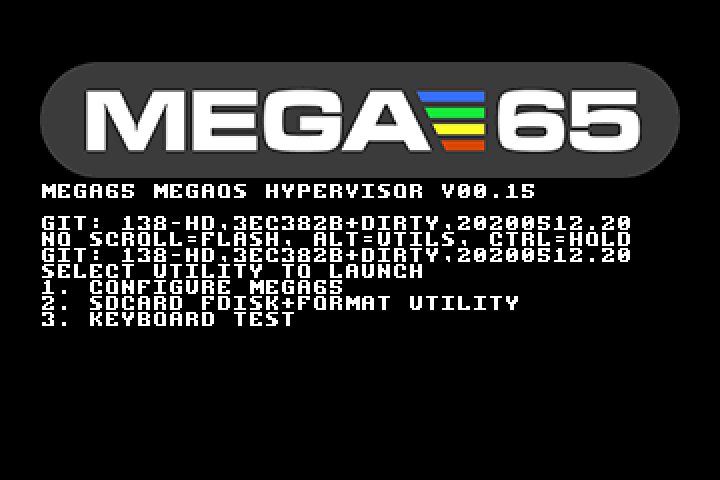
\includegraphics[width=0.7\linewidth]{images/ss-utilmenu.png}
\end{center}

%\begin{minipage}{\linewidth}
  Next, press the number corresponding to the \screentext{CONFIGURE MEGA65} item.  The MEGA65
  Configuration Utility will launch, showing a display similar to
  the following:

%  \vspace{5mm}
\begin{center}
  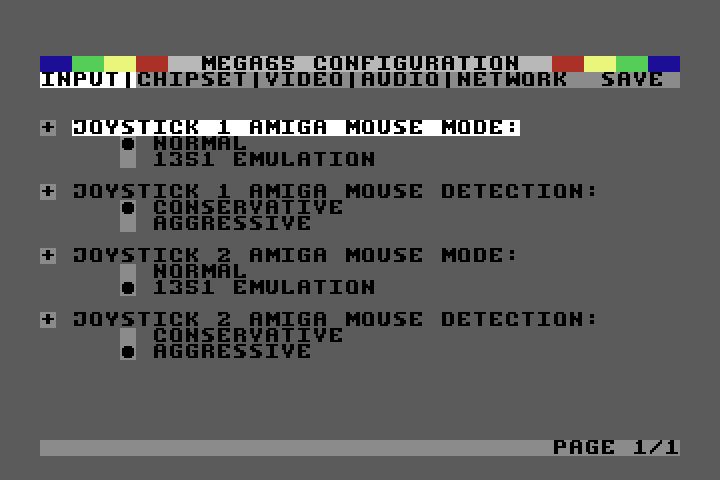
\includegraphics[width=0.7\linewidth]{images/ss-m65config-1.png}
\end{center}
%\end{minipage}

%\begin{minipage}{\linewidth}
  If your MEGA65's System Partition is corrupted, you may be
  prompted to press \megakey{F14} to correct this, (i.e., hold \specialkey{SHIFT} and press
  \megakey{F13}), with a display similar to the following:

%  \vspace{5mm}
\begin{center}
  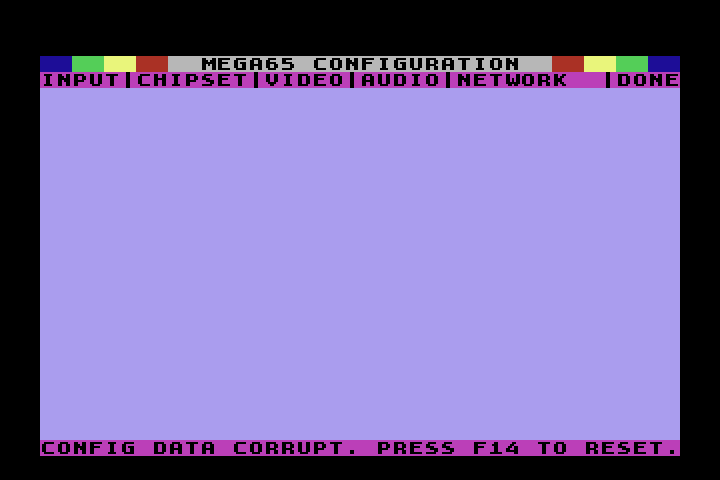
\includegraphics[width=0.7\linewidth]{images/ss-m65config-corrupt.png}
\end{center}
%\end{minipage}

To correct this error, press \megakey{F14}. Next, press \megakey{F7} to save the reset configuration, otherwise the reset data will not be saved to the MEGA65 System
Partition.

Once you have dismissed that display, or if your MEGA65 System Partition is not corrupt, you can begin exploring and adjusting various settings. The program can be controlled using the keyboard, or optionally, a 1351 or Amiga\texttrademark{} mouse.

You can advance screens by pressing \megakey{F1}, or use \megakey{F2} to navigate in the opposite direction. Use \megakey{$\leftarrow$} and \megakey{$\rightarrow$} to navigate between screens.

Use \megakey{$\uparrow$} and \megakey{$\downarrow$} to select an item.

Press \specialkey{RETURN} or \megakey{SPACE} to toggle a setting, or to change a text or numeric value. The black circle next to an option indicates the current selection.

  When you have finished, press \megakey{F7} to see the
  options for saving the changes. This will give you four options:

\begin{center}
  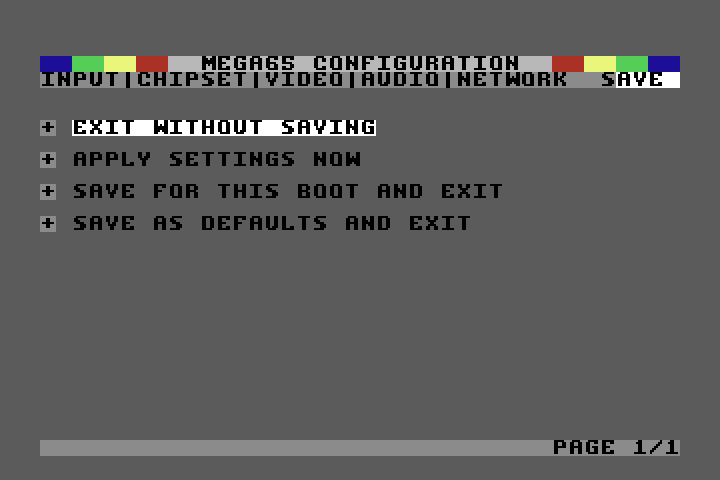
\includegraphics[width=0.7\linewidth]{images/ss-m65config-save.png}
\end{center}

\begin{itemize}
  \item \screentext {EXIT WITHOUT SAVING} abandons any changes made in the MEGA65 Configure utility and exits.
  \item \screentext {APPLY AND TEST SETTINGS NOW} uses the current settings immediately but does not exit. This is helpful to test compatibility of your TV or monitor with PAL or NTSC video modes. If you still see your display after applying a change, it is safe to save those settings.
  \item \screentext {RESTORE FACTORY DEFAULTS} resets the MEGA65 configuration settings to the factory defaults. It will randomly select a new MAC address for models that include an internal Ethernet adaptor. If you wish to commit these changes, you must still save them.
  \item \screentext {SAVE AS DEFAULT AND EXIT} commits changes made to the SD card. These changes will be used when the MEGA65 is switched on.
\end{itemize}

\subsection{Input Devices}

\begin{center}
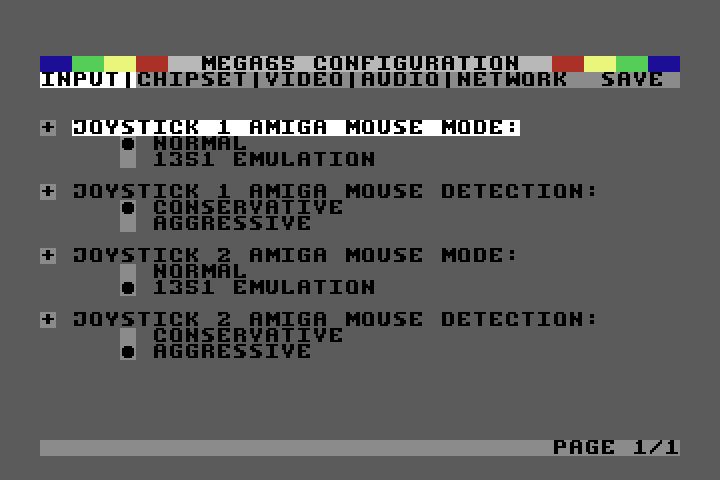
\includegraphics[width=0.7\linewidth]{images/ss-m65config-1.png}
\end{center}

\begin{itemize}
  \item \screentext{JOYSTICK 1 AMIGA MOUSE MODE} allows either \screentext{NORMAL} operation,
  where software will see it as an Amiga mouse or \screentext{1351 EMULATION} mode, where the MEGA65 translates the Amiga mouse's movements into 1351 compatible signals. This allows you to use an Amiga mouse with existing C64/C65 software that expects a 1351 mouse.
  \item \screentext{JOYSTICK 1 AMIGA MOUSE DETECTION} can be set to \screentext{CONSERVATIVE} or \screentext{AGGRESSIVE}. If you use an Amiga mouse and it fails to move smoothly in all directions, you may set it to \screentext{AGGRESSIVE}. Conversely, if you regularly use joysticks in the port, and have difficulties with the joystick input misbehaving, you might want to use the \screentext{CONSERVATIVE} option.
  \item \screentext{JOYSTICK 2 AMIGA MOUSE MODE} is identical to the first option, but for the second controller port. This allows you to have different settings for each port.
  \item \screentext{JOYSTICK 2 AMIGA MOUSE DETECTION} similarly provides the ability to separately control the Amiga mouse detection algorithm for the second controller port.
\end{itemize}


\subsection{Chipset}
\label{configuring-chipset}
\begin{center}
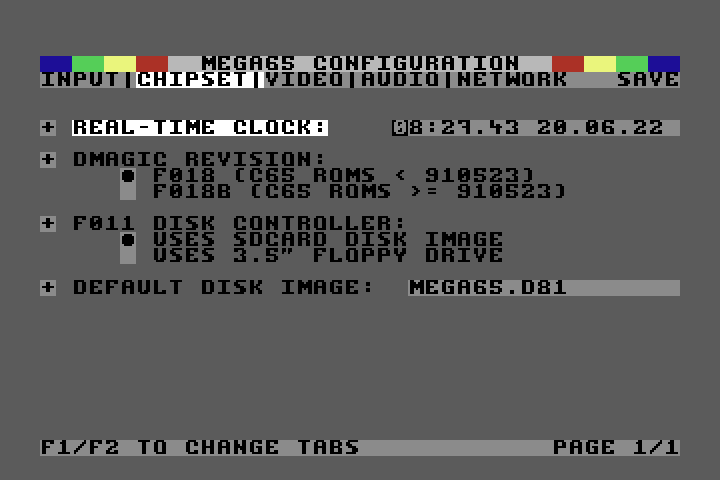
\includegraphics[width=0.7\linewidth]{images/ss-m65config-2.png}
\end{center}

\begin{itemize}
  \item \screentext{REAL-TIME CLOCK} allows setting the MEGA65's Real-Time
    Clock for those models that include one.  To set the clock or
    calendar, simply edit the field and press \specialkey{RETURN}.
    The display does not change while viewing this page, but if
    you use \megakey{$\leftarrow$} and \megakey{$\rightarrow$} to select another page and
    return to this page, the values will update if a Real-Time Clock
    is fitted and functioning.
  \item \screentext{DMAGIC REVISION} allows selecting the default mode of
    operation for the C65 DMAgic DMA controller.  This option is only
    required for ROMs not detected by the MEGA65's HYPPO Hypervisor.
    If you see screen corruption in BASIC,
    try toggling this option.
  \item \screentext{F011 DISK CONTROLLER}
    \index{Disk Drives!D81 Images}
    This option allows you to select whether the internal 3.5'' floppy
    drive functions using real diskettes, or whether it simply makes
    noises to add atmosphere when using D81 disk images from the SD
    card.  This merely sets the default option, and you can change
    this setting, or select a different disk image for use as either
    or both of the C65 3.5'' DOS based drives.
  \item \screentext{DEFAULT DISK IMAGE} allows you to choose the D81 disk image
    used with the internal drive, if the \screentext{F011 DISK CONTROLLER}
    option above is set to \screentext{USES SDCARD DISK IMAGE}. You can read more about
    D81 disk images on page \pageref{sec:d81-images}.
  \item \screentext{LONG FN SUPPORT} is a feature that is still under development
    at time of writing, and we suggest leaving it disabled for now until the feature
    matures in future bitstreams. Its aim is to provide long filename support for the
    SD card.
\end{itemize}

\subsection{Video}

\begin{center}
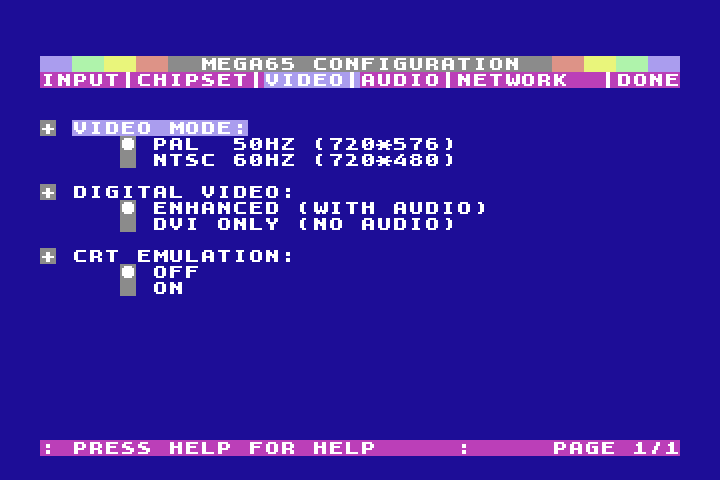
\includegraphics[width=0.7\linewidth]{images/ss-m65config-3.png}
\end{center}
\index{Display!Setting PAL/NTSC}
\begin{itemize}
  \item \screentext{VIDEO MODE} selects whether the MEGA65 starts in PAL or NTSC.    The MEGA65 supports true 480p NTSC and 576p PAL double-scan modes, with exact 60Hz / 50Hz frame-rates. This setting sets the default value, and the system can be switched between PAL and NTSC via the Freeze Menu, or under software control by MEGA65-enabled programs.
  \item \screentext{DIGITAL VIDEO} allows for selection between either \screentext{ENHANCED} video output containing audio, or \screentext{DVI ONLY} video output with no audio.
  \item \screentext{CRT EMULATION} selects whether CRT scanline emulation should be applied to the video output or not.
\end{itemize}

\subsection{Audio}

\begin{center}
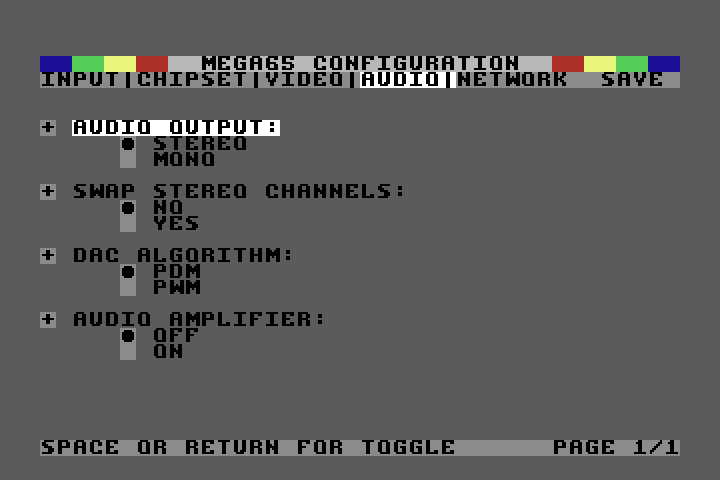
\includegraphics[width=0.7\linewidth]{images/ss-m65config-4.png}
\end{center}

\begin{itemize}
  \item \screentext{AUDIO OUTPUT} selects whether the SIDs and digital audio channels are combined to provide a monaural signal or whether the left and right tagged audio sources are separated to provide a stereo signal. This setting can be changed in the Audio Mixer of the Freeze Menu, or under the control of MEGA65-enabled software.
  \item \screentext{SWAP STEREO CHANNELS} allows switching the left and right-hand sides of the stereo audio output. This is useful for software that expects left and right SIDs to be at swapped addresses compared with the MEGA65 defaults.
  \item \screentext{DAC ALGORITHM} allows selecting between two different digital to analog conversion algorithms. Both options sound good and the selection is a personal preference.
  \item \screentext{AUDIO AMPLIFIER} allows enabling or disabling the audio amplifier contained in some models of the MEGA65. This option works for audio outputs, e.g., internal speaker or loud speaker.
\end{itemize}

\subsection{Network}

\begin{center}
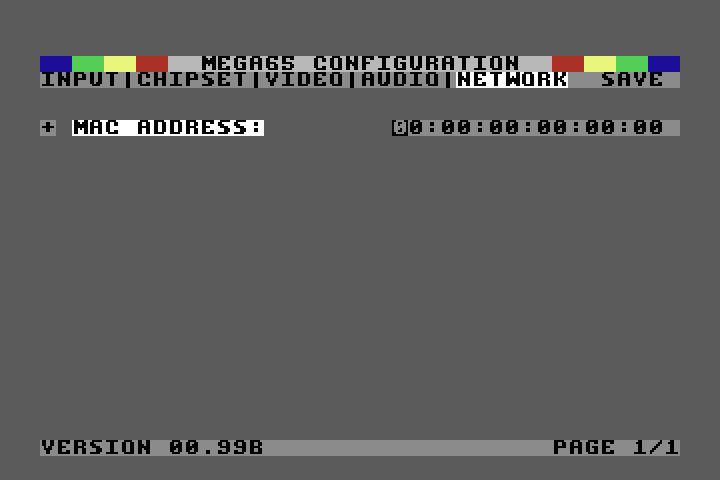
\includegraphics[width=0.7\linewidth]{images/ss-m65config-5.png}
\end{center}

\begin{itemize}
  \item \screentext{MAC ADDRESS} allows you to set the default MAC address of your MEGA65. This can be changed at run-time by MEGA65-enabled software.
\end{itemize}

% 2021-03-17 edits by SBC
